% !TEX root = ../deviant.tex

\section{Experimental evaluation}
\label{sec:eval}

\todoindl{x Fede, Chiara DFM, Sergio: qui bisognerebbe introdurre la metodologia per provare la validit\`a del nostro approccio, cio\`e abbiamo preso questo esempio, abbiamo generato delle tracce, alcune positive, altre negative che per\`o violano dei vincoli che in questo modello non sono presenti e poi abbiamo visto se riusciamo a re-impararli. Perch\`e proprio questi vincoli e non altri?}


\subsection{Motivating example}
A bank carries out the following \emph{loan application} process\footnote{The process is inspired by the Loan Application process reported in (2018, Dumas).} in order to grant loans. The process starts when the \emph{loan application} is received. In order to decide whether to \emph{reject the application} or to \emph{send the acceptance pack} to the customer for receiving the customer's official acceptance, the bank has to \emph{assess} the \emph{eligibility} of the loan. To this aim, the customer's \emph{property} has to be \emph{appraised} and the \emph{loan risk assessed} by the bank. The bank can optionally \emph{notify} the customer about the loan \emph{approval}, of course in case the loan is not rejected. During the process the bank can also \emph{receive positive} or \emph{negative feedback} according to the experience of the loan requester. To ease the understanding of the loan application process, a Declare model of the process is reported in Fig. \ref{fig:ex}\todoindl{x Chiara DFM: La figura non corrisponde esattamente al modello usato da federico. Bisognerebbe: 1. rimuovere not-coexistense tra Send acceptance pack e Reject application. 2. aggiungere not-coexistence tra receive positive feedback e receive negative feedback}.


\begin{figure}[t]
\centering
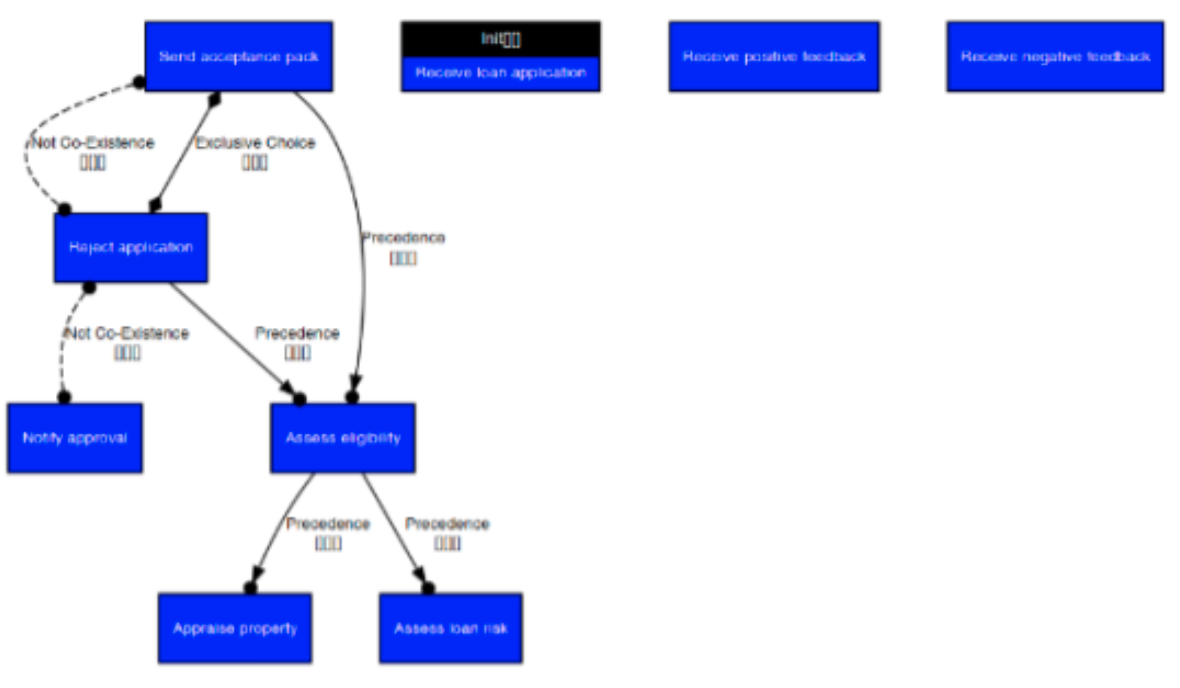
\includegraphics[width=\columnwidth]{example}
\caption{Loan approval declare process model }
\label{fig:ex}
\end{figure}

Among the processed loan application requests, some are considered as negative by the bank, while others as positive. In detail, the negative cases are the ones in which:
\begin{itemize}
\item the bank receives a negative feedback, although the acceptance pack is sent to the customer;
\item the time required for carrying out the whole procedure is huge (this happens when the property appraisal is performed after the loan risk assessment).
\end{itemize}

Being aware of the process executions that deviate from its expectations (the negative cases), the bank would like to discover a process model of the loan application procedure in which only the positive cases are included, while the deviant ones are excluded.


\subsection{Datasets}
\todoindl{x Chiara DFM: questa sezione credo sia da ripopolare da capo perch\`e l'esempio \`e cambiato}

\subsection{Results}

